\section{Моделирование 
  физических процессов,
  протекающих в проектируемом
  радиоэлектронном средстве}

% В данном разделе будет приведены данные о моделировании устройства в
% следующих программах:
% \begin{itemize}
% \item Ansys,
  
% \item COMSOL Multiphysics,
% \item Solidworks Simulation,
  
% \item Solidworks Flow Simulation.
% \end{itemize}

% Будет приведена инфомарция касательно результатов моделирования данных
% программах.

\subsection{Обоснование выбора пакета
 прикладного программного обеспечения 
 SolidWorks Simulation
 для моделирования физических процессов, протекающих в РЭС}

При моделировании физических явлений, протекающих в электронной
аппаратуре при эксплуатации серьёзные требования предъявляются к
точности и адекватности разрабатываемых моделей, к возможностям
программного обеспечения и вычислительным ресурсам

Метод конечных элементов (МКЭ) – основной подход к анализу
напряженно-деформированного состояния, лежащий в основе подавляющего
большинства современных CAE-систем, предназначенных для выполнения
расчётов на прочность различных конструкций посредством численных
алгоритмов. МКЭ используется не только в области прочностных
расчётов, но и для решения задач во многих других сферах, например,
решения задач теплопроводности, гидродинамики, электромагнетизма и др.

В результате анализа САПР, руководствуясь личным опытом работы, для
выполнения моделирования физических процессов были выбрана такое
прикладное программные обеспечение, как SolidWorks Simulation.


Программный продукт SolidWorks является самым распространенным
инструментом, используемым для автоматизированного проектирования и 3D
моделирования. SolidWorks Simulation – это система анализа
конструкций, полностью интегрированная с SolidWorks. Эта система
обеспечивает анализ напряжения, потери устойчивости, оптимизации, а
также частотный и термический анализ на одном экране. Оснащенный
быстрыми решающими программами, SolidWorks Simulation дает возможность
быстро решать большие задачи, используя персональный компьютер.

Популярность SolidWorks Simulation в кругах инженеров позволяет
рассчитывать на наличие большого количества обучающих материалов, в
том числе созданных не только самой компанией осуществляющей
разработку программы.

Кроме того SolidWorks Simulation сам по себе обладают огромным набором
возможностей для проведения симуляции и интегрирует их в интерфейс
параметрического САПР, что позволяет интерактивно взаимодействовать с
геометрией модели, материалом и сеткой модели.

Также особенно хочется отметить доступность и качество документации
доступной на официальном сайте SolidWorks.

Совокупноcть вышеописанных качеств делает эту программы достойным
выбором для проведения исследования.

\subsection{Технология моделирования механических процессов,
протекающих в электронном модуле и устройстве в целом с
использованием  SolidWorks Simulation}

В моделирование механических процессов включает частотный анализ
печатной платы. Эксперимент проводится в среде SolidWorks Simulation.

\begin{figure}[H]
  \centering
  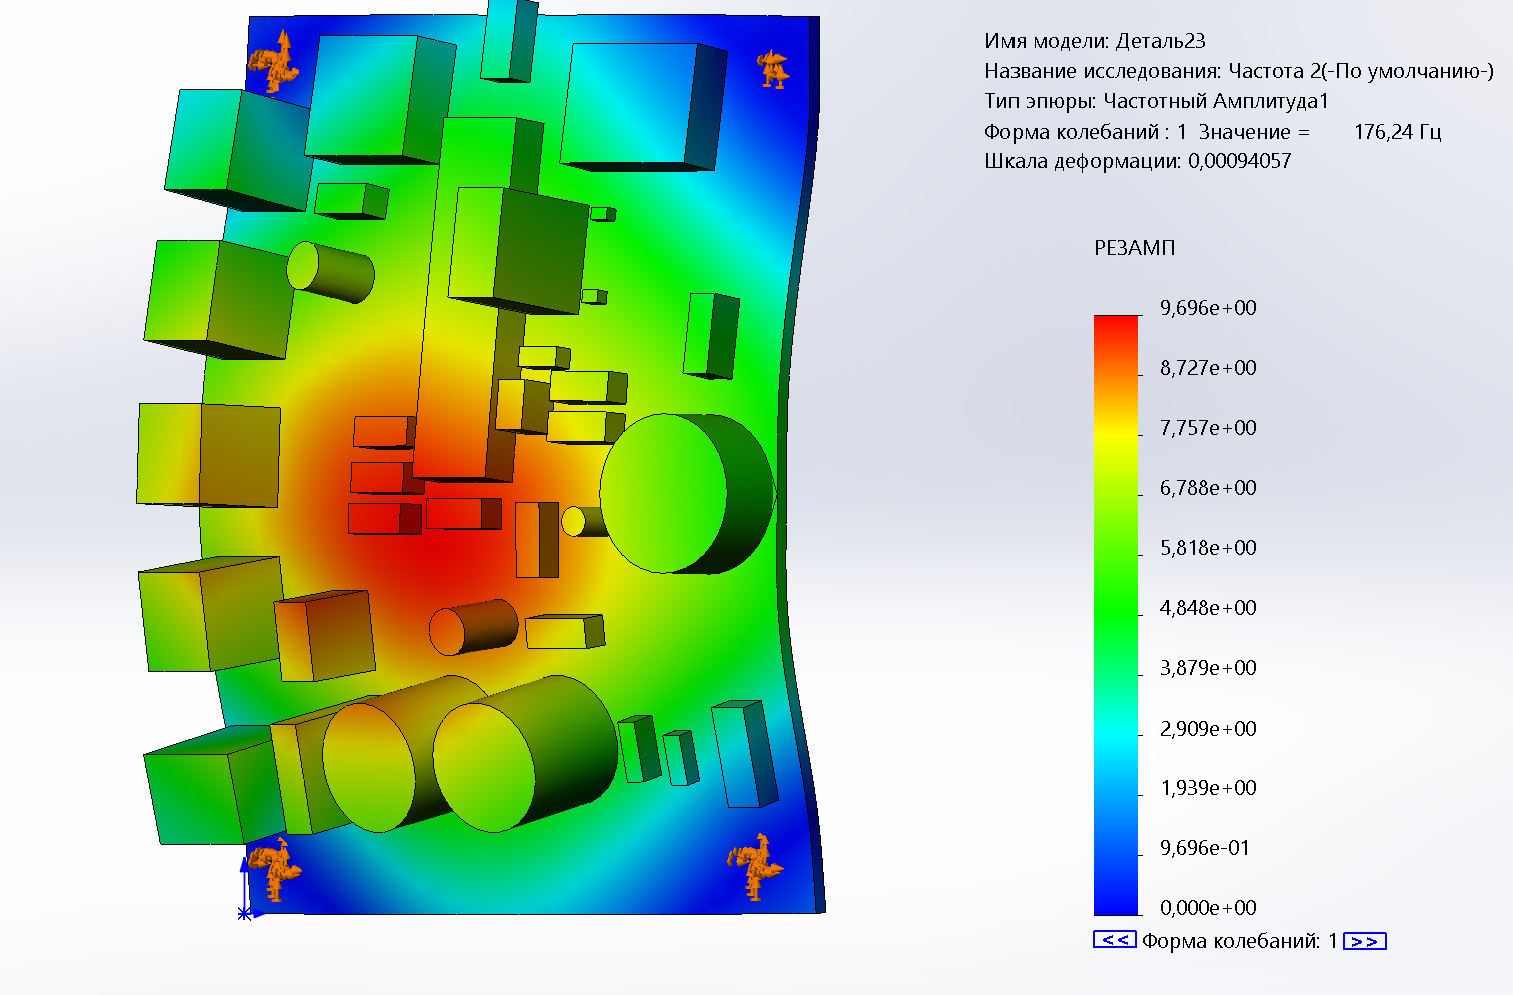
\includegraphics[scale=0.5]{solid.modeling/Amplitude-1-1.png}
  \caption{Результат эксперимента в SolidWorks Simulation (вариант 1)}
\end{figure}

\begin{figure}[H]
  \centering
  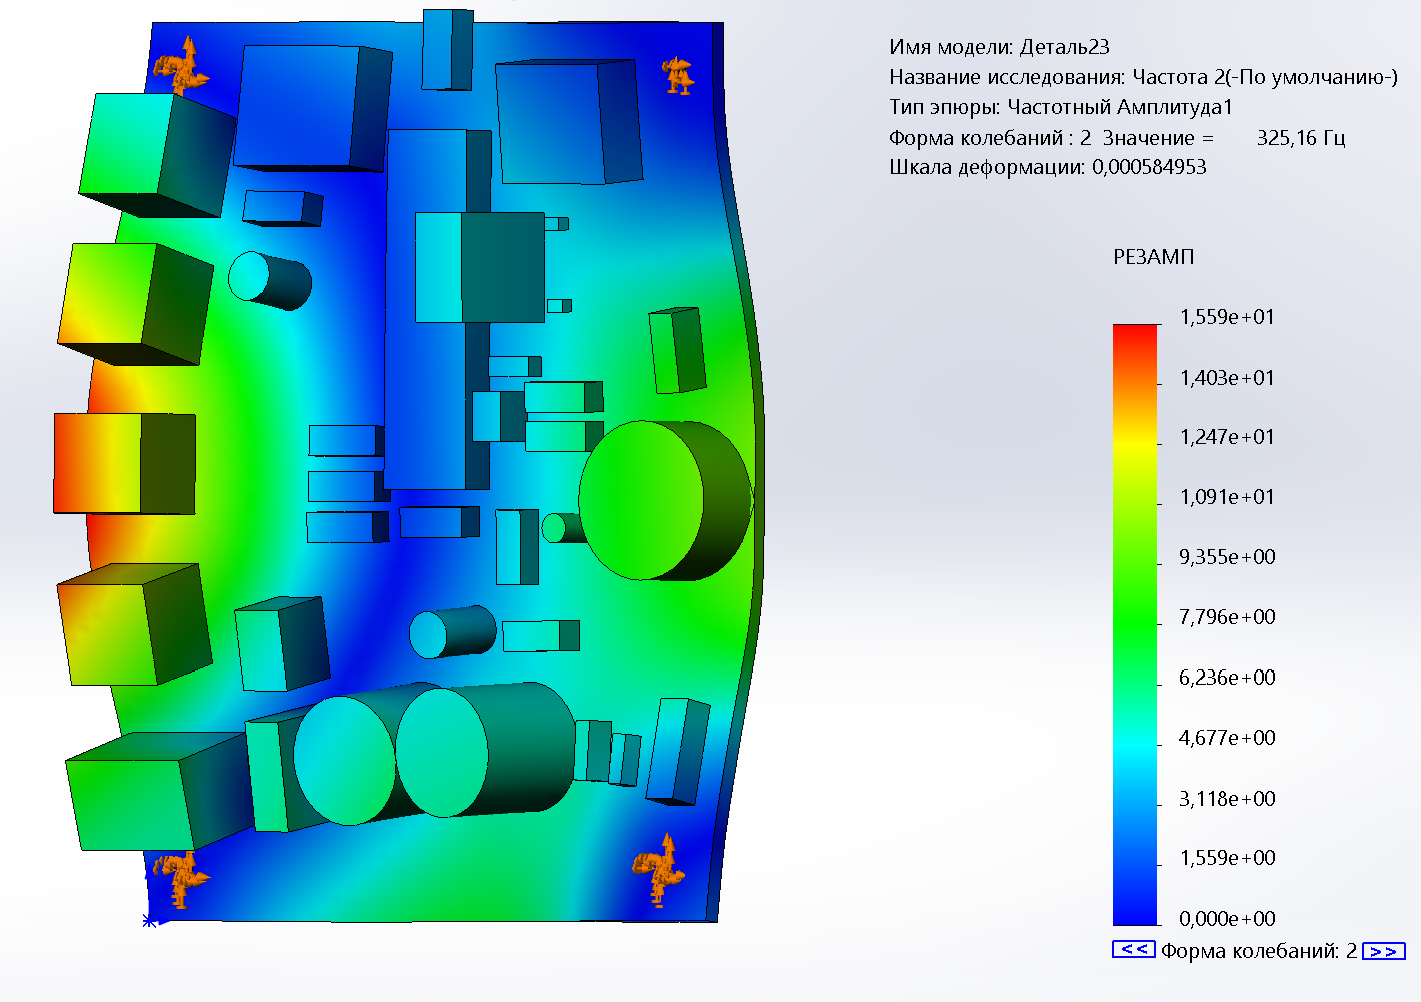
\includegraphics[scale=0.5]{solid.modeling/Amplitude-1-2.png}
  \caption{Результат эксперимента в SolidWorks Simulation (вариант 2)}
\end{figure}

\begin{figure}[H]
  \centering
  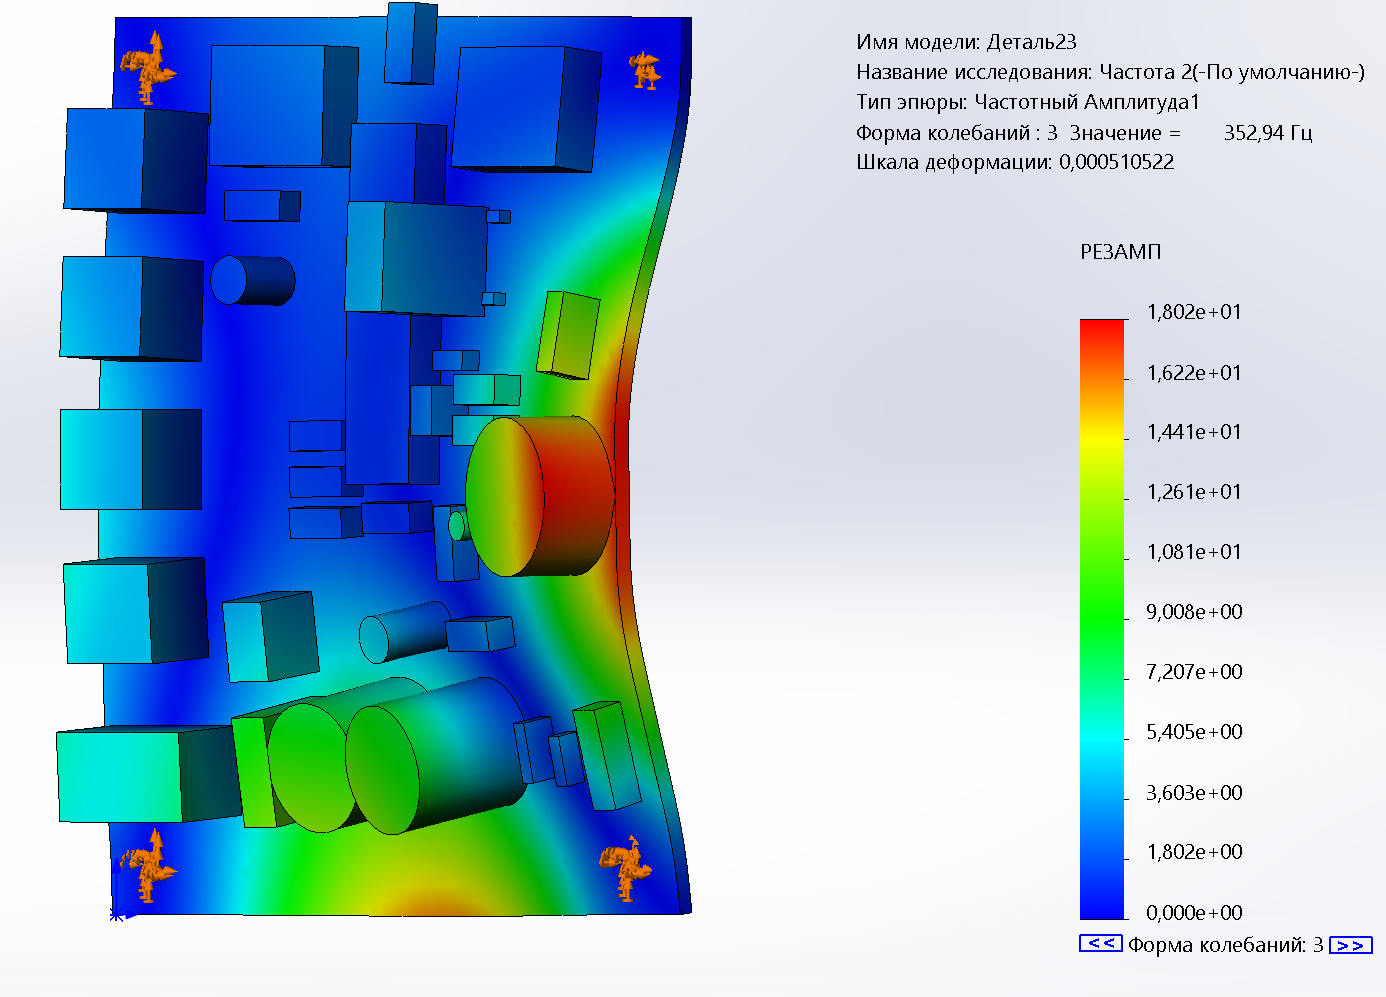
\includegraphics[scale=0.5]{solid.modeling/Amplitude-1-3.png}
  \caption{Результат эксперимента в SolidWorks Simulation (вариант 3)}
\end{figure}

Из результатов моделирования видно, что значения собственных частот
конструкции являются приемлемыми, так как значительно превышают
мак-максимальную воздействующую частоту. Небольшие различия порядка
единиц герц связаны с отличиями между вариантами эксперимента.

\subsection{Обработка, анализ и интерпретация данных результатов
моделирования программными средствами SolidWorks Simulation.}

Данные, полученные в ходе моделирования, собраны вместе и
систематизированы.



\newpage

%%% Local Variables:
%%% mode: LaTeX
%%% TeX-master: "main"
%%% LaTeX-biblatex-use-Biber: t
%%% End:
